% Options for packages loaded elsewhere
\PassOptionsToPackage{unicode}{hyperref}
\PassOptionsToPackage{hyphens}{url}
\PassOptionsToPackage{dvipsnames,svgnames,x11names}{xcolor}
%
\documentclass[
]{agujournal2019}

\usepackage{amsmath,amssymb}
\usepackage{iftex}
\ifPDFTeX
  \usepackage[T1]{fontenc}
  \usepackage[utf8]{inputenc}
  \usepackage{textcomp} % provide euro and other symbols
\else % if luatex or xetex
  \usepackage{unicode-math}
  \defaultfontfeatures{Scale=MatchLowercase}
  \defaultfontfeatures[\rmfamily]{Ligatures=TeX,Scale=1}
\fi
\usepackage{lmodern}
\ifPDFTeX\else  
    % xetex/luatex font selection
\fi
% Use upquote if available, for straight quotes in verbatim environments
\IfFileExists{upquote.sty}{\usepackage{upquote}}{}
\IfFileExists{microtype.sty}{% use microtype if available
  \usepackage[]{microtype}
  \UseMicrotypeSet[protrusion]{basicmath} % disable protrusion for tt fonts
}{}
\makeatletter
\@ifundefined{KOMAClassName}{% if non-KOMA class
  \IfFileExists{parskip.sty}{%
    \usepackage{parskip}
  }{% else
    \setlength{\parindent}{0pt}
    \setlength{\parskip}{6pt plus 2pt minus 1pt}}
}{% if KOMA class
  \KOMAoptions{parskip=half}}
\makeatother
\usepackage{xcolor}
\setlength{\emergencystretch}{3em} % prevent overfull lines
\setcounter{secnumdepth}{5}
% Make \paragraph and \subparagraph free-standing
\makeatletter
\ifx\paragraph\undefined\else
  \let\oldparagraph\paragraph
  \renewcommand{\paragraph}{
    \@ifstar
      \xxxParagraphStar
      \xxxParagraphNoStar
  }
  \newcommand{\xxxParagraphStar}[1]{\oldparagraph*{#1}\mbox{}}
  \newcommand{\xxxParagraphNoStar}[1]{\oldparagraph{#1}\mbox{}}
\fi
\ifx\subparagraph\undefined\else
  \let\oldsubparagraph\subparagraph
  \renewcommand{\subparagraph}{
    \@ifstar
      \xxxSubParagraphStar
      \xxxSubParagraphNoStar
  }
  \newcommand{\xxxSubParagraphStar}[1]{\oldsubparagraph*{#1}\mbox{}}
  \newcommand{\xxxSubParagraphNoStar}[1]{\oldsubparagraph{#1}\mbox{}}
\fi
\makeatother


\providecommand{\tightlist}{%
  \setlength{\itemsep}{0pt}\setlength{\parskip}{0pt}}\usepackage{longtable,booktabs,array}
\usepackage{calc} % for calculating minipage widths
% Correct order of tables after \paragraph or \subparagraph
\usepackage{etoolbox}
\makeatletter
\patchcmd\longtable{\par}{\if@noskipsec\mbox{}\fi\par}{}{}
\makeatother
% Allow footnotes in longtable head/foot
\IfFileExists{footnotehyper.sty}{\usepackage{footnotehyper}}{\usepackage{footnote}}
\makesavenoteenv{longtable}
\usepackage{graphicx}
\makeatletter
\def\maxwidth{\ifdim\Gin@nat@width>\linewidth\linewidth\else\Gin@nat@width\fi}
\def\maxheight{\ifdim\Gin@nat@height>\textheight\textheight\else\Gin@nat@height\fi}
\makeatother
% Scale images if necessary, so that they will not overflow the page
% margins by default, and it is still possible to overwrite the defaults
% using explicit options in \includegraphics[width, height, ...]{}
\setkeys{Gin}{width=\maxwidth,height=\maxheight,keepaspectratio}
% Set default figure placement to htbp
\makeatletter
\def\fps@figure{htbp}
\makeatother
% definitions for citeproc citations
\NewDocumentCommand\citeproctext{}{}
\NewDocumentCommand\citeproc{mm}{%
  \begingroup\def\citeproctext{#2}\cite{#1}\endgroup}
\makeatletter
 % allow citations to break across lines
 \let\@cite@ofmt\@firstofone
 % avoid brackets around text for \cite:
 \def\@biblabel#1{}
 \def\@cite#1#2{{#1\if@tempswa , #2\fi}}
\makeatother
\newlength{\cslhangindent}
\setlength{\cslhangindent}{1.5em}
\newlength{\csllabelwidth}
\setlength{\csllabelwidth}{3em}
\newenvironment{CSLReferences}[2] % #1 hanging-indent, #2 entry-spacing
 {\begin{list}{}{%
  \setlength{\itemindent}{0pt}
  \setlength{\leftmargin}{0pt}
  \setlength{\parsep}{0pt}
  % turn on hanging indent if param 1 is 1
  \ifodd #1
   \setlength{\leftmargin}{\cslhangindent}
   \setlength{\itemindent}{-1\cslhangindent}
  \fi
  % set entry spacing
  \setlength{\itemsep}{#2\baselineskip}}}
 {\end{list}}
\usepackage{calc}
\newcommand{\CSLBlock}[1]{\hfill\break\parbox[t]{\linewidth}{\strut\ignorespaces#1\strut}}
\newcommand{\CSLLeftMargin}[1]{\parbox[t]{\csllabelwidth}{\strut#1\strut}}
\newcommand{\CSLRightInline}[1]{\parbox[t]{\linewidth - \csllabelwidth}{\strut#1\strut}}
\newcommand{\CSLIndent}[1]{\hspace{\cslhangindent}#1}

\usepackage{url} %this package should fix any errors with URLs in refs.
\usepackage{lineno}
\usepackage[inline]{trackchanges} %for better track changes. finalnew option will compile document with changes incorporated.
\usepackage{soul}
\linenumbers
\makeatletter
\@ifpackageloaded{caption}{}{\usepackage{caption}}
\AtBeginDocument{%
\ifdefined\contentsname
  \renewcommand*\contentsname{Table of contents}
\else
  \newcommand\contentsname{Table of contents}
\fi
\ifdefined\listfigurename
  \renewcommand*\listfigurename{List of Figures}
\else
  \newcommand\listfigurename{List of Figures}
\fi
\ifdefined\listtablename
  \renewcommand*\listtablename{List of Tables}
\else
  \newcommand\listtablename{List of Tables}
\fi
\ifdefined\figurename
  \renewcommand*\figurename{Figure}
\else
  \newcommand\figurename{Figure}
\fi
\ifdefined\tablename
  \renewcommand*\tablename{Table}
\else
  \newcommand\tablename{Table}
\fi
}
\@ifpackageloaded{float}{}{\usepackage{float}}
\floatstyle{ruled}
\@ifundefined{c@chapter}{\newfloat{codelisting}{h}{lop}}{\newfloat{codelisting}{h}{lop}[chapter]}
\floatname{codelisting}{Listing}
\newcommand*\listoflistings{\listof{codelisting}{List of Listings}}
\makeatother
\makeatletter
\makeatother
\makeatletter
\@ifpackageloaded{caption}{}{\usepackage{caption}}
\@ifpackageloaded{subcaption}{}{\usepackage{subcaption}}
\makeatother
\ifLuaTeX
  \usepackage{selnolig}  % disable illegal ligatures
\fi
\usepackage{bookmark}

\IfFileExists{xurl.sty}{\usepackage{xurl}}{} % add URL line breaks if available
\urlstyle{same} % disable monospaced font for URLs
\hypersetup{
  pdftitle={Mapping landscape suitability for forest thinning to reduce evapotranspiration and enhance groundwater recharge in Arizona},
  pdfauthor={Ryan E Lima; Temuulen Tsagaan Sankey; Abraham E Springer},
  pdfkeywords={suitability mapping, forest thinning, water
yield, groundwater recharge},
  colorlinks=true,
  linkcolor={blue},
  filecolor={Maroon},
  citecolor={Blue},
  urlcolor={Blue},
  pdfcreator={LaTeX via pandoc}}

\journalname{Water Resources Research}

\draftfalse

\begin{document}
\title{Mapping landscape suitability for forest thinning to reduce
evapotranspiration and enhance groundwater recharge in Arizona}

\authors{Ryan E Lima\affil{1}, Temuulen Tsagaan Sankey\affil{1}, Abraham
E Springer\affil{1}}
\affiliation{1}{Northern Arizona University, }
\correspondingauthor{Ryan E Lima}{ryan.lima@nau.edu}


\begin{abstract}
Here, we review the literature on the effects of forest thinning on
water yield throughout Arizona and map areas where mechanical treatment
has the highest potential for increasing groundwater recharge. This
research synthesizes the myriad studies examining the effects of forest
treatment on water yield in semi-arid forests and compiles a list of
relevant variables. Our approach combines thematic maps of average
precipitation, elevation, slope, aspect, forest type, forest density,
depth to bedrock, and soil type into a GIS suitability model to
highlight areas where forest treatment will most likely enhance recharge
statewide. Rechage in the region is ephemeral and focused in periods of
snowmelt and locations of enhanced permeability when soil moisture
exceeds threshold levels.
\end{abstract}




\section{Introduction}\label{introduction}

Since 2000, the Colorado River Basin has been in the midst of a historic
drought (Meko et al., 2022; Williams et al., 2022). Average temperatures
increased by 0.9ºC from 2000 - 2014, and streamflow in the Colorado
River has declined by 19\% below the 1906-1999 average (Hogan \&
Lundquist, 2024; Udall \& Overpeck, 2017). Extreme hydroclimate events
such as droughts, heatwaves, and floods have more than doubled in
frequency since 2010 (Bennett et al., 2021). Simultaneously, Arizona has
experienced rapid population growth, increasing the demands on already
strained water supplies. Reductions in streamflow have increased
reliance on groundwater pumping, while groundwater levels have declined
for decades in much of the state (Tadych et al., 2024). The average
annual precipitation in the Lower Colorado River Basin is about 330mm,
and only about 10mm of that precipitation becomes streamflow, while much
of the rest is lost to evapotranspiration (Zou et al., 2010).
Sublimation has been shown to remove 10 - 90\% of snowfall in the basin;
the remaining snowmelt provides over 80\% of streamflow to the Colorado
River (Lundquist et al., 2024). Therefore, small reductions in
evaporative losses could have out-sized impacts on available water
supplies (Hibbert, 1979).

Over 90\% of annual precipitation in semi-arid forests can be lost to
evapotranspiration (Dore et al., 2012; Ha et al., 2015; Hibbert, 1979;
Yaseef et al., 2010). Around 65\% of surface water in the western states
originates from forested lands, which cover just 29\% of the land area
(Brown et al., 2005). However, western forests are increasingly at risk
from catastrophic wildfires, an emerging driver of runoff change that
will increase the impact on the water supply (Williams et al., 2022).
Forest structure has changed significantly post-Euro-American settlement
due to grazing, logging, wildfire exclusion, and other factors
(Covington \& Moore, 1994; Friederici, 2013). As a result, many forests
in Arizona are overstocked relative to pre-settlement conditions,
increasing the risk of catastrophic wildfire (Allen et al., 2002).
Rising temperatures and related droughts have contributed to extensive
tree mortality from wildfire, disease, and insect infestation (Berner et
al., 2017). Warming temperatures have tripled the frequency and
quadrupled the size of wildfires in recent decades (Williams et al.,
2022). Increasing heat has pushed many low-elevation conifer forests
past climate thresholds, creating conditions less suitable for tree
regeneration (Davis et al., 2019).

Landscape-scale forest restoration efforts have been planned or
implemented across much of Arizona. For example, the Four Forest
Restoration Initiative (4FRI) includes plans for restoration across over
1 million hectares of Arizona's forests (Schultz et al., 2012). The
primary goal of restoration efforts is to reduce wildfire risk (Allen et
al., 2002; Friederici, 2013). However, numerous studies have linked
forest treatments to increased water yields in semi-arid forests and
have emphasized the role of forest restoration in improving hydrologic
services and increasing water availability (Baker, 1986; Bosch \&
Hewlett, 1982; Gottfried, 1991; Hibbert, 1979; Moreno et al., 2015;
O'Donnell et al., 2018; Schenk et al., 2020; Simonit et al., 2015;
Smerdon et al., 2009; C. Wyatt et al., 2015; C. J. W. Wyatt, 2013; Zou
et al., 2010). Forest treatments such as thinning and burning can
significantly impact the hydrologic cycle of forests (Del Campo et al.,
2022). For example, forest thinning in Arizona has been associated with
increased snow cover days (Belmonte et al., 2021a; Donager et al., 2021;
Sankey et al., 2015), greater soil moisture (Belmonte et al., 2022;
Sankey \& Tatum, 2022), and greater forest canopy moisture (Sankey et
al., 2021). However, the response of forests to treatments is complex
and non-linear and differs across forest types, with treatment level,
and along aspect and elevational gradients (Biederman et al., 2022a; Del
Campo et al., 2022; Hibbert, 1979; Moore \& Wondzell, 2005; Zou et al.,
2010).

Water yield can decrease with reductions in forest cover in drier
forests with little topographic shading or SW aspects due to increased
water use by remaining vegetation and increased snow sublimation or
direct evaporation of soil moisture (Biederman et al., 2015; Goeking \&
Tarboton, 2020). Biederman and others (Biederman et al., 2022a) found
that low-elevation forests in Arizona may produce less streamflow
following reductions in canopy cover due to wildfire, highlighting the
importance of elevation and particularly water-energy asynchrony to
water yield (Webb et al., 2024). The effects of forest treatment appear
to have little or no effect on water yield in areas receiving less than
500mm of annual precipitation (Adams et al., 2012; Biederman et al.,
2022a; Carroll et al., 2016; Hibbert, 1979; Zou et al., 2010).

** Papers on how thinning works primarily in snow-dominated systems**

This research aims to develop criteria for areas suitable for thinning
to enhance groundwater recharge. It focuses primarily on regional
studies to determine suitability criteria, which are likely the best
predictor of hydrologic response to treatment (C. J. W. Wyatt, 2013).

\subsection{Regional Hydrologic Responses to
Treatment}\label{regional-hydrologic-responses-to-treatment}

Several regional studies link forest treatment to changes in stand-level
ecohydrology, including increased tree growth in Ponderosa Pines
(\textbf{Rodman et al., 2024}) greater soil moisture and total ecosystem
moisture leading to increased drought resilience (Sankey et al., 2021;
Sankey \& Tatum, 2022), increased snow retention (Belmonte et al.,
2021b; Broxton et al., 2023), greater streamflow (Baker, 1986), water
table rise {[}Denver et al in Prep {]}{[}Smerdon et al. (2009){]}(Schenk
et al., 2020) and increased springflow (Schenk et al., 2020){[}Hart
prarie and hoxworth in prep{]}.

\subsubsection{Water Yield/Runoff}\label{water-yieldrunoff}

Several regional studies link forest treatment to increased streamflow
(Biederman et al., 2022a; Broxton et al., 2023; Dwivedi et al., 2024).
However, there appears to be a threshold response, with water yield
increasing only in treated forests receiving over 500mm of annual
precipitation or in snow-dominated forests (Adams et al., 2012;
Biederman et al., 2022a; Carroll et al., 2016; Hibbert, 1979; Zou et
al., 2010).

\subsubsection{Soil Moisture and Drought
Resilience}\label{soil-moisture-and-drought-resilience}

A synthesis of several treatment types across Northern Arizona,
including thinning at various levels and prescribed burning, found that
treated sites had significantly greater total ecosystem moisture, making
forests more resilient to drought(Sankey et al., 2021; Sankey \& Tatum,
2022). Treatments were shown to increase tree growth, improving
resilience to drought in Ponderosa Pine forests (\textbf{Rodman et al.,
2024}). Thinned Ponderosa Pine forests have higher soil moisture for two
to eight years post-thinning, a result also found in semi-arid forests
around the Mediterranean (Belmonte et al., 2022; Del Campo et al., 2019,
2022; O'Donnell et al., 2021).

\subsubsection{Justification}\label{justification}

\begin{itemize}
\item
  regional studies are the best predictor of hydrologic response to
  thinning in Arizona forests (C. J. W. Wyatt, 2013)
\item
  A snythesis of all 4FRI treatments found that thinned and burned
  forests have signifiantly greater total ecosystem moisture and are
  thus more resilient to drought and wildfire (Sankey et al., 2021)
\item
  Thinned forests are better buffered against drought impacts in terms
  of both soil moisture and tree health (Sankey \& Tatum, 2022).
\item
  Soil moisture and ET may be affected by thinning for 3.6 - 8.6 years
  (Del Campo et al., 2022).
\item
  Prescribed burning or thinning can increase tree growth, improving
  resilience to drought in ponderosa pine forests (Rodman et al., 2024)
\item
  Thinned forests (around Flagstaff) have higher soil moisture at 25 and
  50cm in the first two years post-thinning (Belmonte et al., 2022).
\item
  Thinning in semi-arid forests around the Mediterranean increased
  antecedent soil moisture and below ground hydrologic processes and
  increased deep soil moisture by 50mm/year over the control (Del Campo
  et al., 2019).
\item
  a review of 35 studies published from 1971 to 2018 found that thinning
  was more effective than clear-cutting in terms of increasing
  groundwater recharge due to reduced sublimation and evaporation.
  Springs can effectively monitor groundwater recharge effects in arid
  lands (Schenk et al., 2020).
\item
  A review of studies on forest mgmt effects on groundwater resources
  found that a rise in the water table can generally be expected
  following forest thinning in all forested landscapes (Smerdon et al.,
  2009).
\end{itemize}

\paragraph{Snow retention}\label{snow-retention}

\begin{itemize}
\item
  The effects of forest thinning and subsequent snowmelt are highly
  variable, with responses depending on forest structure and local
  climate, where thinning in dense and taller vegetation generally
  increases snow retention, thinning in shorter, less dense forests may
  decrease retention (Lewis et al., 2023).
\item
  In semi-arid forested watersheds, thinning can influence streamflow
  variability by modifying snowpack accumulation and melt, particularly
  in wetter years where thinning can either reduce or increase snow
  retention based on site-specific conditions.(Broxton et al., 2023).
\item
  Thinning in semi-arid forested watersheds can significantly impact
  streamflow by altering snowmelt timing, with reduced forest cover
  tending to delay snowmelt at warmer sites while advancing melt at
  cooler, snowpack-persistent sites (Dwivedi et al., 2024).
\item
  Thinned forests around Flagstaff have greater snow persistence at
  25\%-35\% canopy cover (Belmonte et al., 2021a)
\item
  Thinned forests in Northern Arizona have more snow and soil moisture
  (O'Donnell et al., 2021)
\item
  Found that thinned and burned vs.~control forests had varying rates of
  snowmelt and snow persistence. Canopy cover is most predictive of snow
  persistence (Donager et al., 2021).
\end{itemize}

\paragraph{Thresholds in literature}\label{thresholds-in-literature}

\begin{itemize}
\item
  A review of 94 catchment studies showed that significant changes in
  water yield are correlated to forest growth in forests that receive
  600-1200 mm of mean annual precipitation Bosch and Hewlett, 1982 The
  caveat being there were not many coniferous forests studies in that
  precipitation range (Bosch \& Hewlett, 1982).
\item
  (Adams et al., 2012) hypothesized that where annual precipitation
  exceeds \textasciitilde500 mm or water yield is dominated by snowmelt,
  watershed will experience significantly decreased evapotranspiration
  and increased flows if canopy cover is reduced by over 20\%. However,
  their recent observations suggest that in dry forests, water yield may
  decrease. More research is needed. This paper was focused on tree-die
  off not thinning.
\item
  (Carroll et al., 2016) found a threshold hydrologic response when
  evaluating the thinning of a snow-dominated semi-arid Pinyon-Juniper
  community in the Great Basin. They found that a positive water yield
  in thinned plots was only observed when precipitation exceeded 400mm
  annually (wet years)
\item
  (Biederman et al., 2022a) suggests that disturbance will positively
  impact streamflow for a minimum of several years following disturbance
  in areas where mean annual precipitation exceeds \textasciitilde500mm.
  ``Presumably because below 500 mm, most precipitation is evaporated
  regardless of forest condition (Hibbert, 1979){[}@{]}
\item
  (Zhang et al., 2001) evaluated 250 worldwide catchment studies and
  found that the differences in ET between forested and non-forested
  catchments diminish in areas with annual rainfall less than 500 mm
\end{itemize}

\subsubsection{thinning decreases ET in some
circumstances}\label{thinning-decreases-et-in-some-circumstances}

\begin{itemize}
\item
  Reductions of canopy cover can increase ET of existing trees, and
  solar radiation increases ET
  \href{Chen\%20et\%20al.,\%202005;\%20Bennett\%20et\%20al.,\%202018}{@biederman\_recent\_2015}
\item
  Decreases in post-disturbance ET may be offset by increased soil
  evaporation, increasing net ET (Reed et al., 2016)
\item
  (Goeking \& Tarboton, 2020) reviewed the hydrologic response of
  stand-replacing and non-stand-replacing disturbances and found that
  post-disturbance streamflow may increase, not change, or even
  decrease. Non-stand replacing fires---because of increased evaporation
  from higher sub-canopy radiation and increased transpiration from
  rapid post-disturbance growth can reduce water availability in some
  cases.
\end{itemize}

\subsection{Data \& Methods}\label{sec-data-methods}

\subsubsection{Weighted Suitability
Workflow}\label{weighted-suitability-workflow}

\paragraph{Define}\label{define}

\begin{quote}
``define the goal, supporting criteria, and evaluation metrics for the
weighted suitability model.''
\end{quote}

\textbf{Here we define the goal of this suitability map--to locate areas
on the Mogollon Rim Ranger District in the Coconino National Forest
where thinning may increase groundwater recharge based on modeling of
criteria found in the literature quantifying the impact of thinning on
water yield in Regional studies of Semi-arid forests.}

\paragraph{Suitability Criteria}\label{suitability-criteria}

\subparagraph{Aspect}\label{aspect}

Aspect has a large impact on solar radiation.

\begin{quote}
Closer to 0 or 360 is desired, low suitability scores for closeness
\end{quote}

\begin{figure}[H]

{\centering 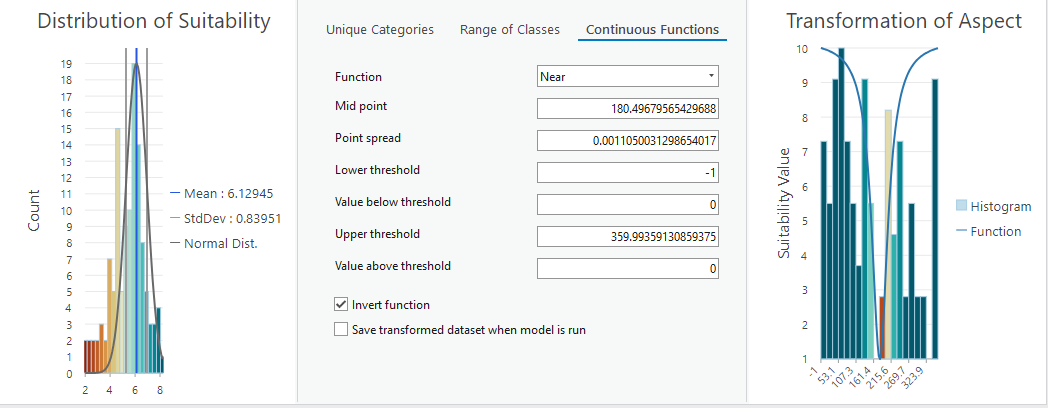
\includegraphics{images/Aspect_suitability.PNG}

}

\caption{Screenshot of Transfer function for Aspect Suitability}

\end{figure}%

\begin{center}\rule{0.5\linewidth}{0.5pt}\end{center}

\subparagraph{Slope}\label{slope}

Higher slopes are less suitable because thinning is both more expensive,
and more precipitation will end up as runoff.

\begin{quote}
Lower slopes have higher suitability scores
\end{quote}

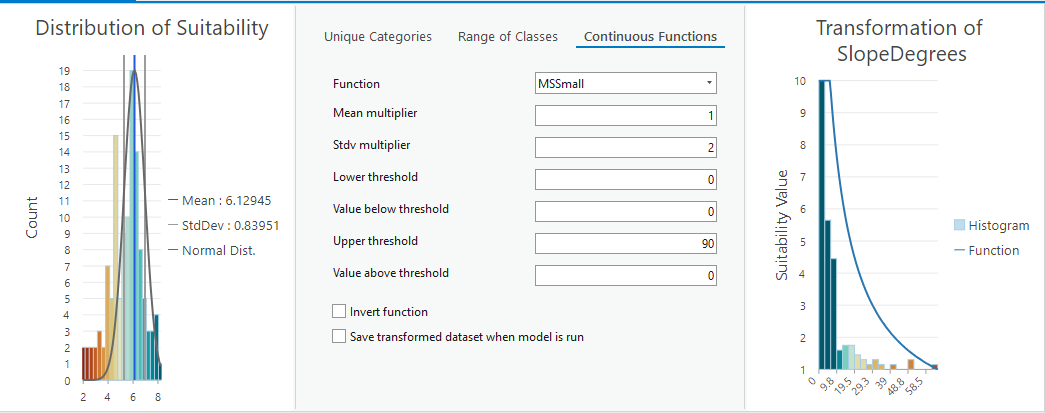
\includegraphics{images/Slope_suitability.PNG}

\begin{center}\rule{0.5\linewidth}{0.5pt}\end{center}

\subparagraph{Elevation}\label{elevation}

Water yield in lower elevation watersheds will be less responsive to
changes in forest structure due to asynchrony between snowmelt and
transpiration (Biederman et al., 2022b)

Winter precipitation mainly falls as snow at elevations above 1800m in
Arizona (Friederici, 2013)

\begin{center}\rule{0.5\linewidth}{0.5pt}\end{center}

\subparagraph{Precipitation}\label{precipitation}

\begin{quote}
\textbf{Ideal:} Mean annual precipitation must be higher than 500mm 1990
- 2020

\textbf{Marginal:} (benefits only expected in wet years or during some
events) Max precipitation higher than 500mm but Mean annual
precipitation \textless{} 500mm

\textbf{Unsuitable:} Max annual precipitation \textless{} 500mm
\end{quote}

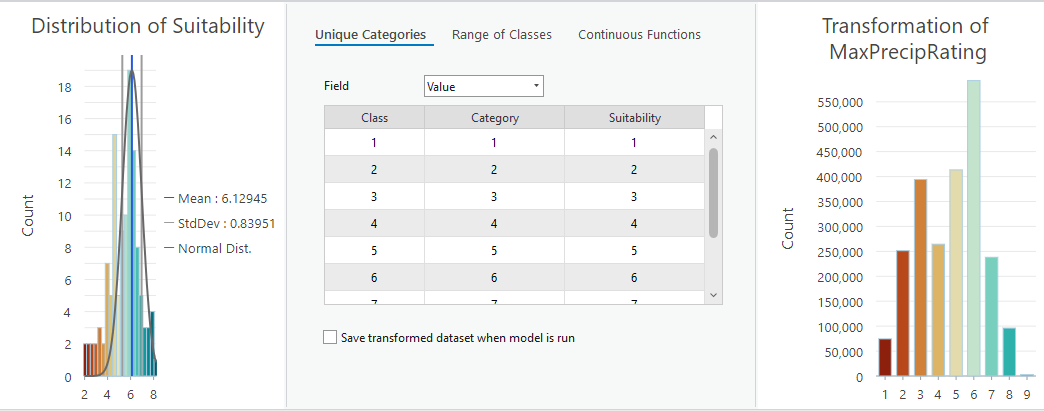
\includegraphics{images/Precipitation_suitability.PNG}

\begin{center}\rule{0.5\linewidth}{0.5pt}\end{center}

\subparagraph{Vegetation
Characteristics}\label{vegetation-characteristics}

Higher vegetation density, when thinned, will yield more water, so focus
on areas of high vegetation density and high departure from historic
conditions.

\begin{quote}
\textbf{NLCD 2021 Total Canopy Cover (\% Cover)}
\end{quote}

\begin{quote}
Canopy cover \% below 30 were considered low suitability (1) while
increases in canopy cover about 30\% increase in suitability.
\end{quote}

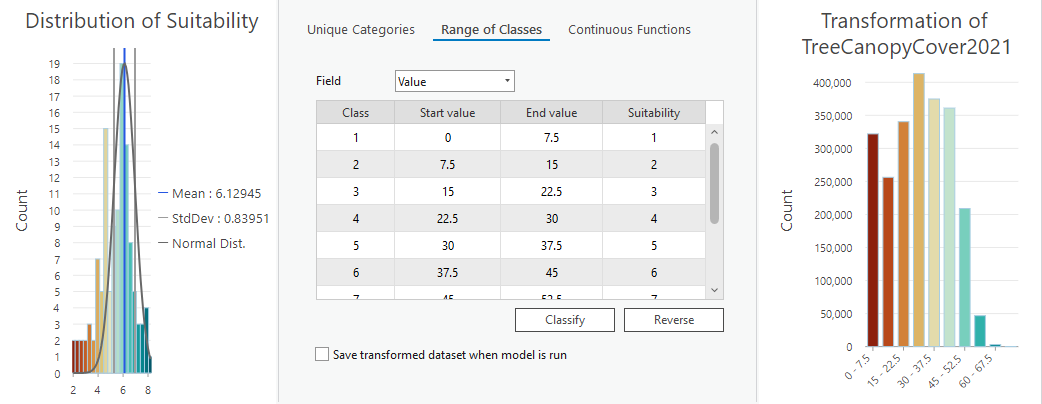
\includegraphics{images/CanopyCover_suitability.PNG}

\begin{quote}
\textbf{Landfire 2022 Vegetation Condition Class} 3rd update to the 2016
remap.
\end{quote}

Variation from modeled historic conditions. Forests that have deviated
significantly from their modeled historic conditions are more suitable
for thinning than forests that have not deviated from their historic
condition.

\begin{quote}
Vegetation Condition Class (VCC) represents a simple categorization of
the associated Vegetation Departure (VDep) and is a derivative of the
VDep layer. It indicates the general level to which current vegetation
differs from the estimated modeled vegetation based on past reference
conditions. VDep and VCC are based upon methods originally described in
the Inter-agency Fire Regime Condition Class Guidebook but are not
identical to those methods. They should not be considered as a
replacement data set. Full descriptions of the techniques used can be
found in the VDep product description. Note that the LANDFIRE (LF) team
feels it is very important for users to review the VDep methods before
comparing VDep or VCC values across LF versions.
\href{https://www.landfire.gov/vegetation/vcc}{info}
\href{https://www.landfire.gov/sites/default/files/DataDictionary/LF2022/LF22_VCCADD_230.pdf}{PDF}
\end{quote}

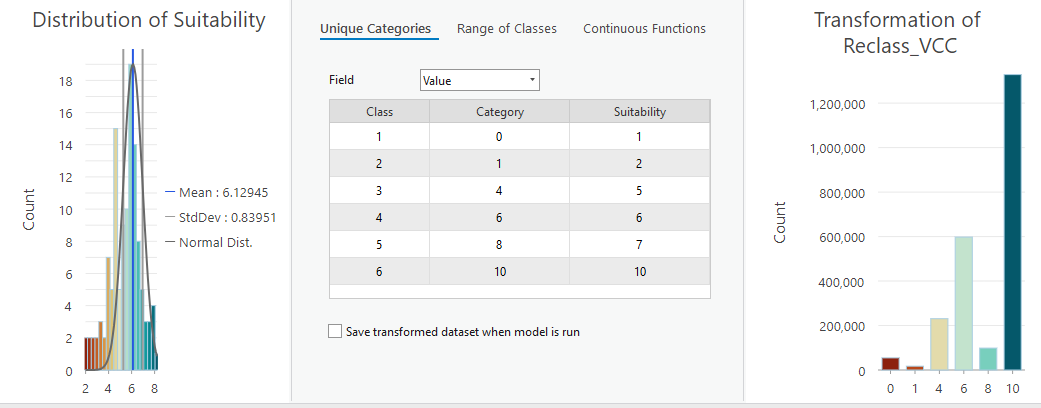
\includegraphics{images/VCC_suitability.PNG}

\begin{center}\rule{0.5\linewidth}{0.5pt}\end{center}

\subparagraph{Soil Hydrologic
Conditions}\label{soil-hydrologic-conditions}

Soil types A,B,C,D are mapped for the USA, There are no A soil types in
the study area, so they were given the following suitability values

B = 10 out of 10 C = 8 out of 10 D = 3 out of 10

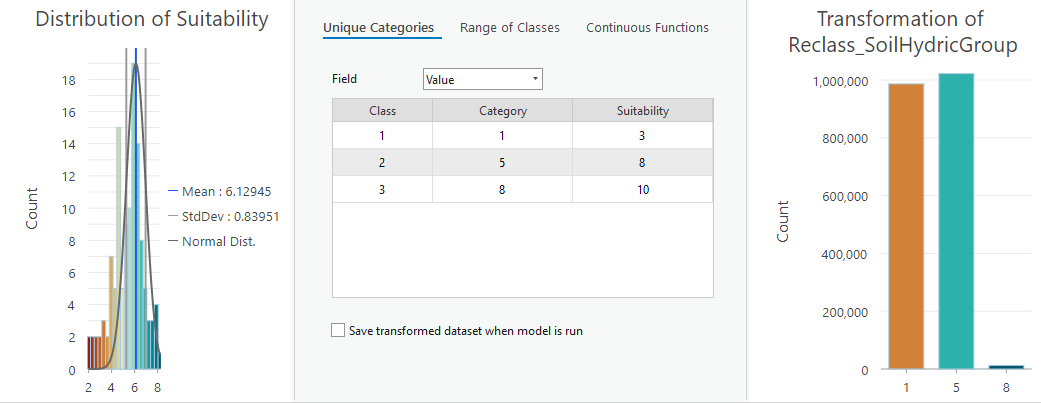
\includegraphics{images/SoilHydrologicGroup_suitability.PNG}

\subsection{Preliminary Results}\label{preliminary-results}

\subsubsection{Weighting}\label{weighting}

Tree Canopy Cover = 20\% Vegetation Condition Class = 20\% Slope = 20\%
Aspect = 20\% Max Precipitation = 15\% Soil Hydrologic Group = 5\%

\subsubsection{Overall Suitability}\label{overall-suitability}

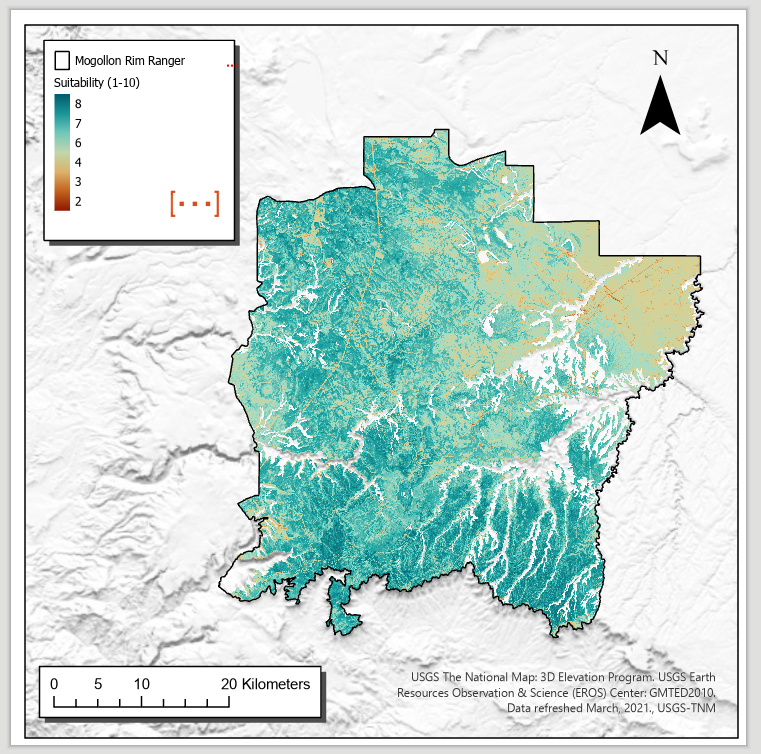
\includegraphics{images/PreliminarySuitabilityMap.PNG}

\subsection{Acknowledgments}\label{acknowledgments}

Phasellus interdum tincidunt ex, a euismod massa pulvinar at. Ut
fringilla ut nisi nec volutpat. Morbi imperdiet congue tincidunt.
Vivamus eget rutrum purus. Etiam et pretium justo. Donec et egestas sem.
Donec molestie ex sit amet viverra egestas. Nullam justo nulla,
fringilla at iaculis in, posuere non mauris. Ut eget imperdiet elit.

\subsection{Open research}\label{open-research}

Phasellus interdum tincidunt ex, a euismod massa pulvinar at. Ut
fringilla ut nisi nec volutpat. Morbi imperdiet congue tincidunt.
Vivamus eget rutrum purus. Etiam et pretium justo. Donec et egestas sem.
Donec molestie ex sit amet viverra egestas. Nullam justo nulla,
fringilla at iaculis in, posuere non mauris. Ut eget imperdiet elit.

\subsection*{References}\label{references}
\addcontentsline{toc}{subsection}{References}

\phantomsection\label{refs}
\begin{CSLReferences}{1}{0}
\vspace{1em}

\bibitem[\citeproctext]{ref-adams_ecohydrological_2012}
Adams, H. D., Luce, C. H., Breshears, D. D., Allen, C. D., Weiler, M.,
Hale, V. C., et al. (2012). Ecohydrological consequences of drought‐ and
infestation‐ triggered tree die‐off: Insights and hypotheses.
\emph{Ecohydrology}, \emph{5}(2), 145--159.
\url{https://doi.org/10.1002/eco.233}

\bibitem[\citeproctext]{ref-allen_ecological_2002}
Allen, C. D., Savage, M., Falk, D. A., Suckling, K. F., Swetnam, T. W.,
Schulke, T., et al. (2002). Ecological restoration of southwestern
ponderosa pine ecosystems: A broad perspective. \emph{Ecological
Applications}, \emph{12}(5), 1418--1433.
\url{https://doi.org/10.1890/1051-0761(2002)012\%5B1418:EROSPP\%5D2.0.CO;2}

\bibitem[\citeproctext]{ref-baker_effects_1986}
Baker, M. B. (1986). Effects of {Ponderosa} {Pine} {Treatments} on
{Water} {Yield} in {Arizona}. \emph{Water Resources Research},
\emph{22}(1), 67--73. \url{https://doi.org/10.1029/WR022i001p00067}

\bibitem[\citeproctext]{ref-belmonte_uav-based_2021}
Belmonte, A., Sankey, T., Biederman, J., Bradford, J., Goetz, S., \&
Kolb, T. (2021a). {UAV}-{Based} {Estimate} of {Snow} {Cover} {Dynamics}:
{Optimizing} {Semi}-{Arid} {Forest} {Structure} for {Snow}
{Persistence}. \emph{Remote Sensing}, \emph{13}(5), 1036.
\url{https://doi.org/10.3390/rs13051036}

\bibitem[\citeproctext]{ref-belmonte2021}
Belmonte, A., Sankey, T., Biederman, J., Bradford, J., Goetz, S., \&
Kolb, T. (2021b). UAV-Based Estimate of Snow Cover Dynamics: Optimizing
Semi-Arid Forest Structure for Snow Persistence. \emph{Remote Sensing},
\emph{13}(5), 1036. \url{https://doi.org/10.3390/rs13051036}

\bibitem[\citeproctext]{ref-belmonte_soil_2022}
Belmonte, A., Ts. Sankey, T., Biederman, J., Bradford, J. B., \& Kolb,
T. (2022). Soil moisture response to seasonal drought conditions and
post‐thinning forest structure. \emph{Ecohydrology}, \emph{15}(5),
e2406. \url{https://doi.org/10.1002/eco.2406}

\bibitem[\citeproctext]{ref-bennett_concurrent_2021}
Bennett, K. E., Talsma, C., \& Boero, R. (2021). Concurrent {Changes} in
{Extreme} {Hydroclimate} {Events} in the {Colorado} {River} {Basin}.
\emph{Water}, \emph{13}(7), 978. \url{https://doi.org/10.3390/w13070978}

\bibitem[\citeproctext]{ref-berner_tree_2017}
Berner, L. T., Law, B. E., Meddens, A. J. H., \& Hicke, J. A. (2017).
Tree mortality from fires, bark beetles, and timber harvest during a hot
and dry decade in the western {United} {States} (2003--2012).
\emph{Environmental Research Letters}, \emph{12}(6), 065005.
\url{https://doi.org/10.1088/1748-9326/aa6f94}

\bibitem[\citeproctext]{ref-biederman_recent_2015}
Biederman, J. A., Somor, A. J., Harpold, A. A., Gutmann, E. D.,
Breshears, D. D., Troch, P. A., et al. (2015). Recent tree die‐off has
little effect on streamflow in contrast to expected increases from
historical studies. \emph{Water Resources Research}, \emph{51}(12),
9775--9789. \url{https://doi.org/10.1002/2015WR017401}

\bibitem[\citeproctext]{ref-biederman_streamflow_2022}
Biederman, J. A., Robles, M. D., Scott, R. L., \& Knowles, J. F.
(2022a). Streamflow {Response} to {Wildfire} {Differs} {With} {Season}
and {Elevation} in {Adjacent} {Headwaters} of the {Lower} {Colorado}
{River} {Basin}. \emph{Water Resources Research}, \emph{58}(3),
e2021WR030687. \url{https://doi.org/10.1029/2021WR030687}

\bibitem[\citeproctext]{ref-biederman2022}
Biederman, J. A., Robles, M. D., Scott, R. L., \& Knowles, J. F.
(2022b). Streamflow Response to Wildfire Differs With Season and
Elevation in Adjacent Headwaters of the Lower Colorado River Basin.
\emph{Water Resources Research}, \emph{58}(3), e2021WR030687.
\url{https://doi.org/10.1029/2021WR030687}

\bibitem[\citeproctext]{ref-bosch_review_1982}
Bosch, J. M., \& Hewlett, J. D. (1982). A review of catchment
experiments to determine the effect of vegetation changes on water yield
and evapotranspiration. \emph{Journal of Hydrology}, \emph{55}(1-4),
3--23. \url{https://doi.org/10.1016/0022-1694(82)90117-2}

\bibitem[\citeproctext]{ref-brown_source_2005}
Brown, T. C., Hobbins, M. T., \& Ramirez, J. A. (2005). \emph{The
{Source} of {Water} {Supply} in the {United} {States}} (Discussion
\{Paper\} No. RMRS-RWU-4851) (p. 57). Fort Collins, CO: U.S. Department
of Agriculture, Forest Service, Rocky Mountain Research Station.
Retrieved from
\url{https://www.researchgate.net/profile/Jorge-Ramirez-14/publication/266272409_The_source_of_water_supply_in_the_United_States/links/54b5fcb50cf26833efd34687/The-source-of-water-supply-in-the-United-States.pdf}

\bibitem[\citeproctext]{ref-broxton_subseasonal_2023}
Broxton, P. D., Van Leeuwen, W. J. D., Svoma, B. M., Walter, J., \&
Biederman, J. A. (2023). Subseasonal to seasonal streamflow forecasting
in a semiarid watershed. \emph{JAWRA Journal of the American Water
Resources Association}, \emph{59}(6), 1493--1510.
\url{https://doi.org/10.1111/1752-1688.13147}

\bibitem[\citeproctext]{ref-carroll_evaluating_2016}
Carroll, R. W. H., Huntington, J. L., Snyder, K. A., Niswonger, R. G.,
Morton, C., \& Stringham, T. K. (2016). Evaluating mountain meadow
groundwater response to {Pinyon}‐{Juniper} and temperature in a great
basin watershed. \emph{Ecohydrology}, \emph{10}(1), e1792.
\url{https://doi.org/10.1002/eco.1792}

\bibitem[\citeproctext]{ref-covington_southwestern_1994}
Covington, W. W., \& Moore, M. M. (1994). Southwestern ponderosa pine
forest structure: Changes since {Euro}-{American} settlement.
\emph{Journal of Forestry.}, \emph{92}, 39--47.

\bibitem[\citeproctext]{ref-davis_wildfires_2019}
Davis, K. T., Dobrowski, S. Z., Higuera, P. E., Holden, Z. A., Veblen,
T. T., Rother, M. T., et al. (2019). Wildfires and climate change push
low-elevation forests across a critical climate threshold for tree
regeneration. \emph{Proceedings of the National Academy of Sciences},
\emph{116}(13), 6193--6198.
\url{https://doi.org/10.1073/pnas.1815107116}

\bibitem[\citeproctext]{ref-del_campo_effectiveness_2019}
Del Campo, A. D., González-Sanchis, M., Molina, A. J., García-Prats, A.,
Ceacero, C. J., \& Bautista, I. (2019). Effectiveness of water-oriented
thinning in two semiarid forests: {The} redistribution of increased net
rainfall into soil water, drainage and runoff. \emph{Forest Ecology and
Management}, \emph{438}, 163--175.
\url{https://doi.org/10.1016/j.foreco.2019.02.020}

\bibitem[\citeproctext]{ref-del_campo_global_2022}
Del Campo, A. D., Otsuki, K., Serengil, Y., Blanco, J. A., Yousefpour,
R., \& Wei, X. (2022). A global synthesis on the effects of thinning on
hydrological processes: {Implications} for forest management.
\emph{Forest Ecology and Management}, \emph{519}, 120324.
\url{https://doi.org/10.1016/j.foreco.2022.120324}

\bibitem[\citeproctext]{ref-donager_integrating_2021}
Donager, J., Sankey, T. Ts., Sánchez Meador, A. J., Sankey, J. B., \&
Springer, A. (2021). Integrating airborne and mobile lidar data with
{UAV} photogrammetry for rapid assessment of changing forest snow depth
and cover. \emph{Science of Remote Sensing}, \emph{4}, 100029.
\url{https://doi.org/10.1016/j.srs.2021.100029}

\bibitem[\citeproctext]{ref-dore_recovery_2012}
Dore, S., Montes‐Helu, M., Hart, S. C., Hungate, B. A., Koch, G. W.,
Moon, J. B., et al. (2012). Recovery of ponderosa pine ecosystem carbon
and water fluxes from thinning and stand‐replacing fire. \emph{Global
Change Biology}, \emph{18}(10), 3171--3185.
\url{https://doi.org/10.1111/j.1365-2486.2012.02775.x}

\bibitem[\citeproctext]{ref-dwivedi_how_2024}
Dwivedi, R., Biederman, J. A., Broxton, P. D., Pearl, J. K., Lee, K.,
Svoma, B. M., et al. (2024). How three-dimensional forest structure
regulates the amount and timing of snowmelt across a climatic gradient
of snow persistence. \emph{Frontiers in Water}, \emph{6}, 1374961.
\url{https://doi.org/10.3389/frwa.2024.1374961}

\bibitem[\citeproctext]{ref-friederici2013}
Friederici, P. (2013). \emph{Ecological Restoration of Southwestern
Ponderosa Pine Forests}. Chicago: Island Press.

\bibitem[\citeproctext]{ref-goeking_forests_2020}
Goeking, S. A., \& Tarboton, D. G. (2020). Forests and {Water} {Yield}:
{A} {Synthesis} of {Disturbance} {Effects} on {Streamflow} and
{Snowpack} in {Western} {Coniferous} {Forests}. \emph{Journal of
Forestry}, \emph{118}(2), 172--192.
\url{https://doi.org/10.1093/jofore/fvz069}

\bibitem[\citeproctext]{ref-gottfried_moderate_1991}
Gottfried, G. J. (1991). Moderate timber harvesting increases water
yields from an {Arizona} {Mixed} {Conifer} {Watershed}. \emph{JAWRA
Journal of the American Water Resources Association}, \emph{27}(3),
537--546. Retrieved from
\url{https://onlinelibrary.wiley.com/doi/abs/10.1111/j.1752-1688.1991.tb01454.x}

\bibitem[\citeproctext]{ref-ha_evapotranspiration_2015}
Ha, W., Kolb, T. E., Springer, A. E., Dore, S., O'Donnell, F. C.,
Martinez Morales, R., et al. (2015). Evapotranspiration comparisons
between eddy covariance measurements and meteorological and
remote‐sensing‐based models in disturbed ponderosa pine forests.
\emph{Ecohydrology}, \emph{8}(7), 1335--1350.
\url{https://doi.org/10.1002/eco.1586}

\bibitem[\citeproctext]{ref-hibbert1979}
Hibbert, A. R. (1979). \emph{Managing vegetation to increase flow in the
colorado river basin}.

\bibitem[\citeproctext]{ref-hogan_recent_2024}
Hogan, D., \& Lundquist, J. D. (2024). Recent {Upper} {Colorado} {River}
{Streamflow} {Declines} {Driven} by {Loss} of {Spring} {Precipitation}.
\emph{Geophysical Research Letters}, \emph{51}(16), e2024GL109826.
\url{https://doi.org/10.1029/2024GL109826}

\bibitem[\citeproctext]{ref-lewis_prediction_2023}
Lewis, G., Harpold, A., Krogh, S. A., Broxton, P., \& Manley, P. N.
(2023). The prediction of uneven snowpack response to forest thinning
informs forest restoration in the central {Sierra} {Nevada}.
\emph{Ecohydrology}, \emph{16}(7), e2580.
\url{https://doi.org/10.1002/eco.2580}

\bibitem[\citeproctext]{ref-lundquist_sublimation_2024}
Lundquist, J. D., Vano, J., Gutmann, E., Hogan, D., Schwat, E.,
Haugeneder, M., et al. (2024). Sublimation of {Snow}. \emph{Bulletin of
the American Meteorological Society}, \emph{105}(6), E975--E990.
\url{https://doi.org/10.1175/BAMS-D-23-0191.1}

\bibitem[\citeproctext]{ref-meko_treering_2022}
Meko, D. M., Woodhouse, C. A., \& Winitsky, A. G. (2022). Tree‐{Ring}
{Perspectives} on the {Colorado} {River}: {Looking} {Back} and {Moving}
{Forward}. \emph{JAWRA Journal of the American Water Resources
Association}, \emph{58}(5), 604--621.
\url{https://doi.org/10.1111/1752-1688.12989}

\bibitem[\citeproctext]{ref-moore_physical_2005}
Moore, R., \& Wondzell, S. M. (2005). Physical hydrology and the effects
of forest harvesting in the pacific northwest: {A} review. \emph{Journal
of the American Water Resources Association}, \emph{41}(4), 763--784.
\url{https://doi.org/10.1111/j.1752-1688.2005.tb04463.x}

\bibitem[\citeproctext]{ref-moreno_modeling_2015}
Moreno, H. A., Gupta, H. V., White, D. D., \& Sampson, D. A. (2015,
October). Modeling the distributed effects of forest thinning on the
long-term water balance and stream flow extremes for a semi-arid basin
in the southwestern {US}.
\url{https://doi.org/10.5194/hessd-12-10827-2015}

\bibitem[\citeproctext]{ref-odonnell_forest_2018}
O'Donnell, F. C., Flatley, W. T., Springer, A. E., \& Fulé, P. Z.
(2018). Forest restoration as a strategy to mitigate climate impacts on
wildfire, vegetation, and water in semiarid forests. \emph{Ecological
Applications}, \emph{28}(6), 1459--1472.
\url{https://doi.org/10.1002/eap.1746}

\bibitem[\citeproctext]{ref-odonnell_vegetation_2021}
O'Donnell, F. C., Donager, J., Sankey, T., Masek Lopez, S., \& Springer,
A. E. (2021). Vegetation structure controls on snow and soil moisture in
restored ponderosa pine forests. \emph{Hydrological Processes},
\emph{35}(11), e14432. \url{https://doi.org/10.1002/hyp.14432}

\bibitem[\citeproctext]{ref-sankey_thinning_2022}
Sankey, T., \& Tatum, J. (2022). Thinning increases forest resiliency
during unprecedented drought. \emph{Scientific Reports}, \emph{12}(1),
9041. \url{https://doi.org/10.1038/s41598-022-12982-z}

\bibitem[\citeproctext]{ref-sankey_multi-scale_2015}
Sankey, T., Donald, J., McVay, J., Ashley, M., O'Donnell, F., Lopez, S.
M., \& Springer, A. (2015). Multi-scale analysis of snow dynamics at the
southern margin of the {North} {American} continental snow distribution.
\emph{Remote Sensing of Environment}, \emph{169}, 307--319.
\url{https://doi.org/10.1016/j.rse.2015.08.028}

\bibitem[\citeproctext]{ref-sankey_regionalscale_2021}
Sankey, T., Belmonte, A., Massey, R., \& Leonard, J. (2021).
Regional‐scale forest restoration effects on ecosystem resiliency to
drought: A synthesis of vegetation and moisture trends on {Google}
{Earth} {Engine}. \emph{Remote Sensing in Ecology and Conservation},
\emph{7}(2), 259--274. \url{https://doi.org/10.1002/rse2.186}

\bibitem[\citeproctext]{ref-schenk_impacts_2020}
Schenk, E. R., O'Donnell, F., Springer, A. E., \& Stevens, L. E. (2020).
The impacts of tree stand thinning on groundwater recharge in aridland
forests. \emph{Ecological Engineering}, \emph{145}, 105701.
\url{https://doi.org/10.1016/j.ecoleng.2019.105701}

\bibitem[\citeproctext]{ref-schultz_collaborative_2012}
Schultz, C. A., Jedd, T., \& Beam, R. D. (2012). The {Collaborative}
{Forest} {Landscape} {Restoration} {Program}: {A} {History} and
{Overview} of the {First} {Projects}. \emph{Journal of Forestry},
\emph{110}(7), 381--391. \url{https://doi.org/10.5849/jof.11-082}

\bibitem[\citeproctext]{ref-simonit_impact_2015}
Simonit, S., Connors, J. P., Yoo, J., Kinzig, A., \& Perrings, C.
(2015). The {Impact} of {Forest} {Thinning} on the {Reliability} of
{Water} {Supply} in {Central} {Arizona}. \emph{PLOS ONE}, \emph{10}(4),
e0121596. \url{https://doi.org/10.1371/journal.pone.0121596}

\bibitem[\citeproctext]{ref-smerdon_overview_2009}
Smerdon, B. D., Redding, T., \& Beckers, J. (2009). An overview of the
effects of forest management on groundwater hydrology. \emph{Journal of
Ecosystems and Management}.
\url{https://doi.org/10.22230/jem.2009v10n1a409}

\bibitem[\citeproctext]{ref-tadych_historical_2024}
Tadych, D. E., Ford, M., Colby, B. G., \& Condon, L. E. (2024).
Historical patterns of well drilling and groundwater depth in {Arizona}
considering groundwater regulation and surface water access. \emph{JAWRA
Journal of the American Water Resources Association}, 1752--1688.13234.
\url{https://doi.org/10.1111/1752-1688.13234}

\bibitem[\citeproctext]{ref-udall_twentyfirst_2017}
Udall, B., \& Overpeck, J. (2017). The twenty‐first century {Colorado}
{River} hot drought and implications for the future. \emph{Water
Resources Research}, \emph{53}(3), 2404--2418.
\url{https://doi.org/10.1002/2016WR019638}

\bibitem[\citeproctext]{ref-webb2024}
Webb, R., Knowles, John~F., Fox, A., Fabricus, A., Corrie, T., Mooney,
K., et al. (2024). Energy{-}Water Asynchrony Principally Determines
Water Available for Runoff From Snowmelt in Continental Montane Forests.
\emph{Hydrological Processes}, \emph{38}(10).
\url{https://doi.org/10.1002/hyp.15297}

\bibitem[\citeproctext]{ref-williams_rapid_2022}
Williams, A. P., Cook, B. I., \& Smerdon, J. E. (2022). Rapid
intensification of the emerging southwestern {North} {American}
megadrought in 2020--2021. \emph{Nature Climate Change}, \emph{12}(3),
232--234. \url{https://doi.org/10.1038/s41558-022-01290-z}

\bibitem[\citeproctext]{ref-wyatt_semiarid_2015}
Wyatt, C., O'Donnell, F. C., \& Abraham E. Springer. (2015). Semi‐{Arid}
{Aquifer} {Responses} to {Forest} {Restoration} {Treatments} and
{Climate} {Change}. \emph{Ground Water}.
\url{https://doi.org/10.1111/gwat.12184}

\bibitem[\citeproctext]{ref-wyatt_estimating_2013}
Wyatt, C. J. W. (2013). \emph{Estimating groundwater yield following
forest restoration along the {Mogollon} {Rim}} (Master's thesis).
Northern Arizona University, Flagstaff, AZ. Retrieved from
\url{https://cdm17192.contentdm.oclc.org/digital/collection/p17192coll1/id/476/rec/3}

\bibitem[\citeproctext]{ref-yaseef_ecohydrology_2010}
Yaseef, N. R., Yakir, D., Rotenberg, E., Schiller, G., \& Cohen, S.
(2010). Ecohydrology of a semi‐arid forest: Partitioning among water
balance components and its implications for predicted precipitation
changes. \emph{Ecohydrology}, \emph{3}(2), 143--154.
\url{https://doi.org/10.1002/eco.65}

\bibitem[\citeproctext]{ref-zhang_response_2001}
Zhang, L., Dawes, W. R., \& Walker, G. R. (2001). Response of mean
annual evapotranspiration to vegetation changes at catchment scale.
\emph{Water Resources Research}, \emph{37}(3), 701--708.
\url{https://doi.org/10.1029/2000WR900325}

\bibitem[\citeproctext]{ref-zou_streamflow_2010}
Zou, C. B., Ffolliott, P. F., \& Wine, M. (2010). Streamflow responses
to vegetation manipulations along a gradient of precipitation in the
{Colorado} {River} {Basin}. \emph{Forest Ecology and Management},
\emph{259}(7), 1268--1276.
\url{https://doi.org/10.1016/j.foreco.2009.08.005}

\end{CSLReferences}



\end{document}
